\documentclass[a4paper,12pt]{article}
\usepackage[utf8]{inputenc}
\usepackage[cm,empty]{fullpage}
\usepackage[T2A]{fontenc}
\usepackage[english, russian]{babel}
\usepackage{amssymb,amsmath,amsxtra,amsthm}
\usepackage{proof}
\usepackage[pdftex]{graphicx}
\usepackage{wrapfig}
\usepackage{braket}
\usepackage{xcolor}

\usepackage[left=2cm,right=2cm,
    top=1cm,bottom=1cm,bindingoffset=0cm]{geometry}

\renewcommand{\leq}{\leqslant}
\renewcommand{\geq}{\geqslant}


\newcommand{\iiff}{\Longleftrightarrow}
\renewcommand{\iff}{\Leftrightarrow}
\newcommand{\nothing}{\varnothing}

\newtheorem*{rem}{Замечание}

\newcommand{\NN}{\mathbb{N}}
\newcommand{\ZZ}{\mathbb{Z}}
\newcommand{\Q}{\mathbb{Q}}
\newcommand{\A}{\mathbb{A}}
\newcommand{\R}{\mathbb{R}}
\renewcommand{\C}{\mathbb{C}}

\renewcommand{\phi}{\varphi}
\newcommand{\eps}{\varepsilon}

\newcounter{z}


\newcommand{\zs}{\refstepcounter{z}\vskip 10pt\par\noindent
\fbox{\textbf{12.\arabic{z}}} }

\newcommand{\z}{\refstepcounter{z}\vskip 20pt\noindent
\fbox{\textbf{\arabic{z}}} }

\renewcommand{\date}{{\bf 8 марта 2021}} 

\newcommand{\dif}
{
------------------------------------------------------------------------------------------------------------------------------------------------------
}

\newcommand{\HSEhat}{
\vspace*{-0pt}
\noindent
\setcounter{z}{0}


{\bf \phantom{\date}  \large \hfill Математический анализ: \hfill \normalsize \date}

\vspace{5 pt}
{\bf \large \hfill  лекция 4\hfill }

\vspace{15 pt}
\centerline{ \large  Домашнее задание.}
\centerline{ \large  Кирилл Сетдеков}



\vspace*{10pt}
\setcounter{z}{0}

}

\begin{document}
\HSEhat



\begin{enumerate}
\item Задача 1


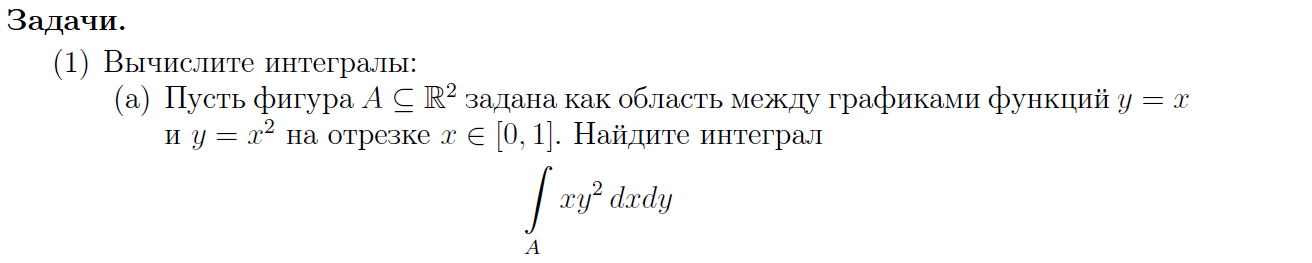
\includegraphics[width=\textwidth]{img/1a.png}

\textbf{Решение:}\\
Запишем как последовательный интеграл:

$$\int_{0}^{1} \int_{y}^{\sqrt{y}} yx^2 dxdy =\int_{0}^{1}  1/2y^2x^2 \Biggr|_{y}^{\sqrt{y}}  dy  =\int_{0}^{1}  1/2y^3- 1/2y^4  dy =\frac{x^4}{8} - \frac{x^5}{10} \Biggr|_{0}^{1}=1/8-1/10=\frac{1}{40}$$

\textbf{Ответ: $\frac{1}{40}$}

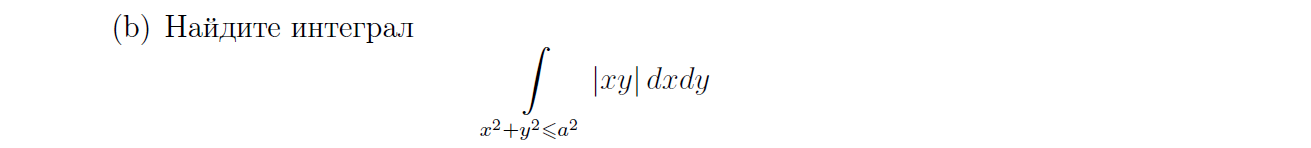
\includegraphics[width=\textwidth]{img/1b.png}
\textbf{Решение:}\\
Из-за знака x и y и того, что значения $|xy|$ одинаково себя ведут в каждой четверти координатной плоскости, будем считать только четверть этого интеграла в положительных значениях x и y и умножим результат на 4. Обозначим искомый ответ как $V$ и будем искать $M=V/4$

$$M = \int_{0}^{a} \int_{0}^{\sqrt{a^2-y^2}} xy dxdy$$

посчитаем внутренний интеграл:
$$\int_{0}^{\sqrt{a^2-y^2}} xy dx = \frac{1}{2}x^2y\Biggr|_{0}^{\sqrt{a^2-y^2}}= \frac{1}{2}y(a^2-y^2)-0= \frac{1}{2}a^2y-\frac{1}{2}y^3$$

$$M = \int_{0}^{a} \frac{1}{2}a^2y-\frac{1}{2}y^3 dy=  \frac{1}{4}a^2y^2-\frac{1}{8}y^4\Biggr|_{0}^{a} = \frac{1}{4}a^2a^2-\frac{1}{8}a^4=\frac{1}{8}a^4$$

$$V=4M = \frac{1}{2}a^4$$
\textbf{Ответ: $\frac{1}{2}a^4$}


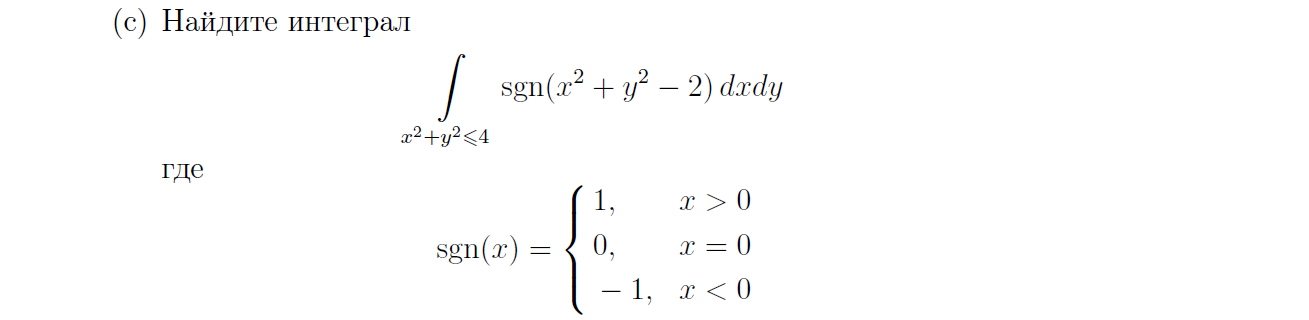
\includegraphics[width=\textwidth]{img/1c.png}
\textbf{Решение:}\\

Функция под интегралом принимает значение +1 вне круга радиусом $\sqrt{2}$ и -1 внутри этого круга. При этом границы интегрирования - это круг радиусом 2. Визуально, можно разложить задачу на нахождение 2 интегралов: $A=B-2S$, где A- искомый результат, B - интеграл 1 по внешней границе, а S - интеграл 1 по границе круга с радиусом $\sqrt{2}$.

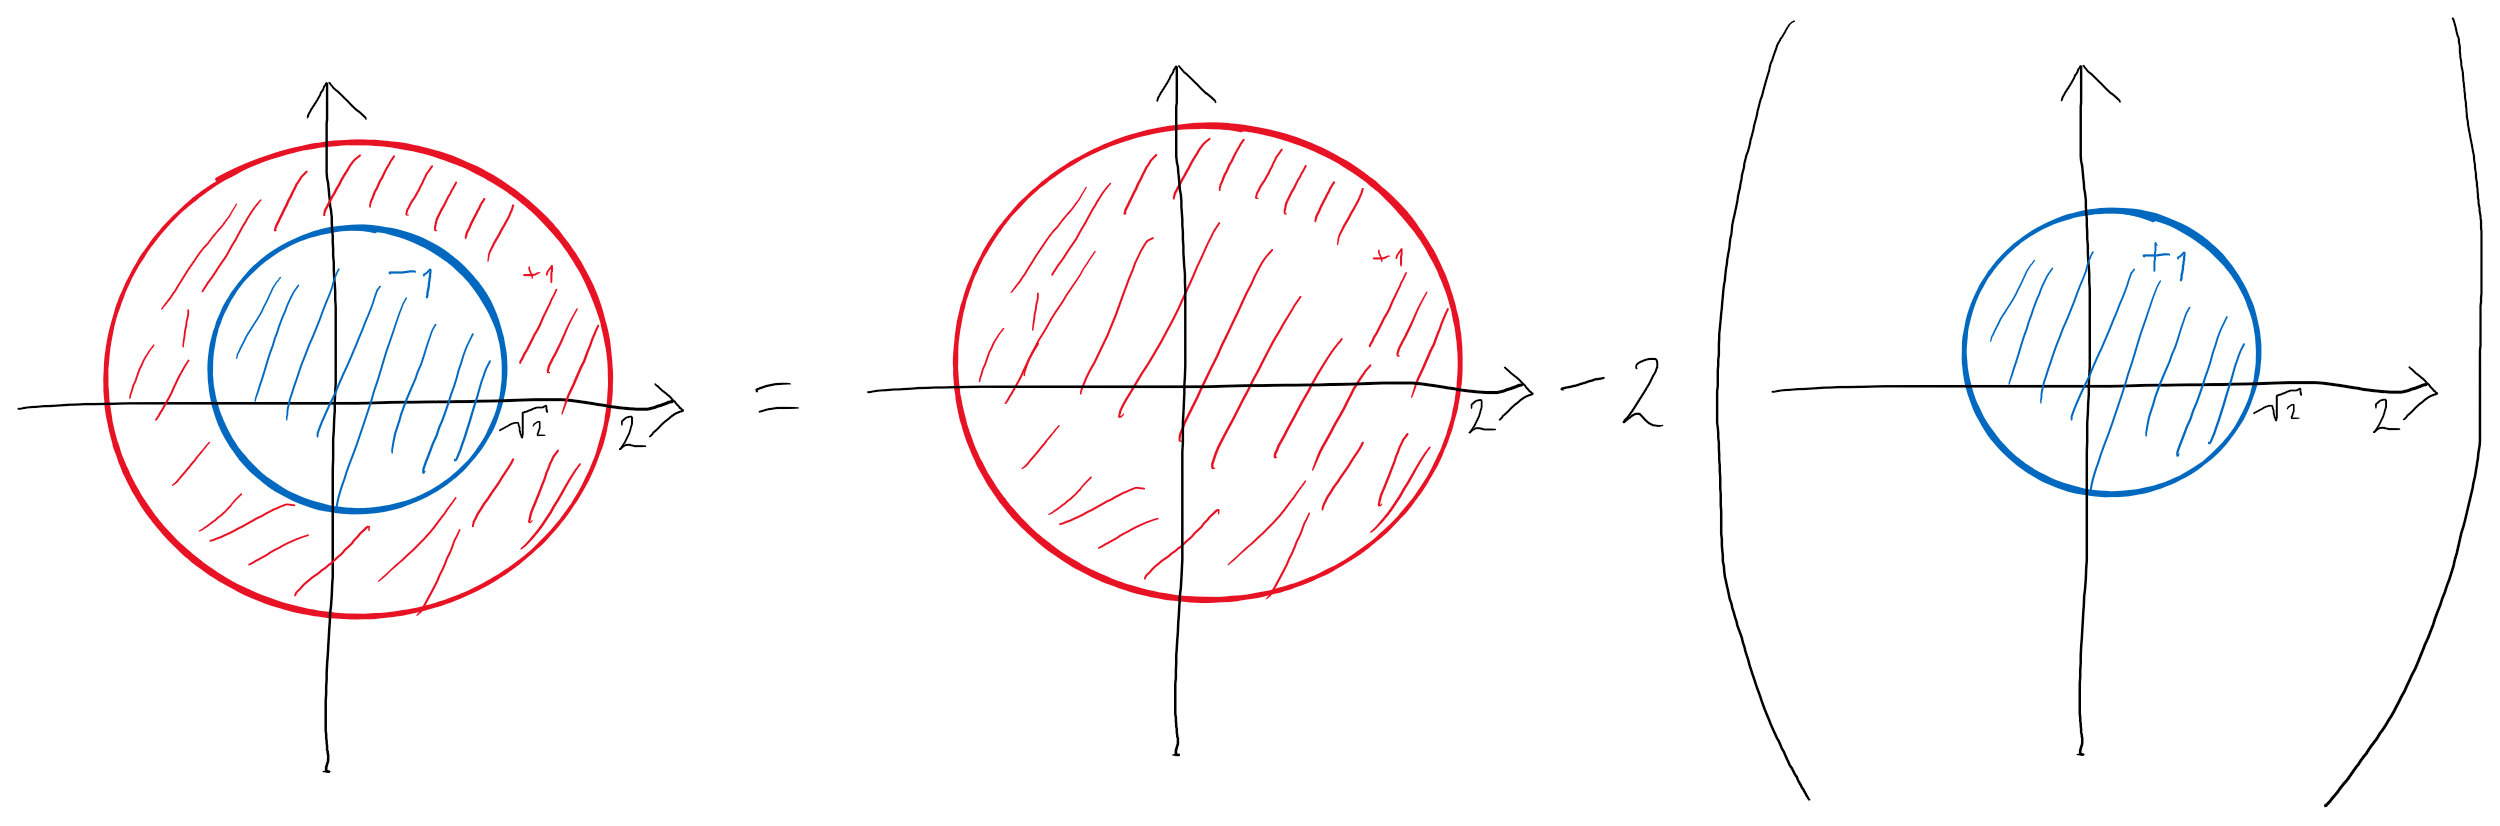
\includegraphics[width=\textwidth]{img/1csolve.png}
Мы знаем, что $\iint_{x^2+y^2\leq R^2} 1 dx dy = \pi R^2$
Следовательно $B = 4\pi$, $S = 2\pi$ а ответ будет $A=B-2S = 4\pi-4\pi=0$

\textbf{Ответ: $0$}


\item вычислите интегралы
\begin{enumerate}
\item 
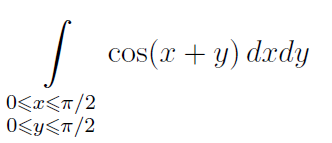
\includegraphics[scale=0.5]{img/2a.PNG}

\textbf{Решение:}\\
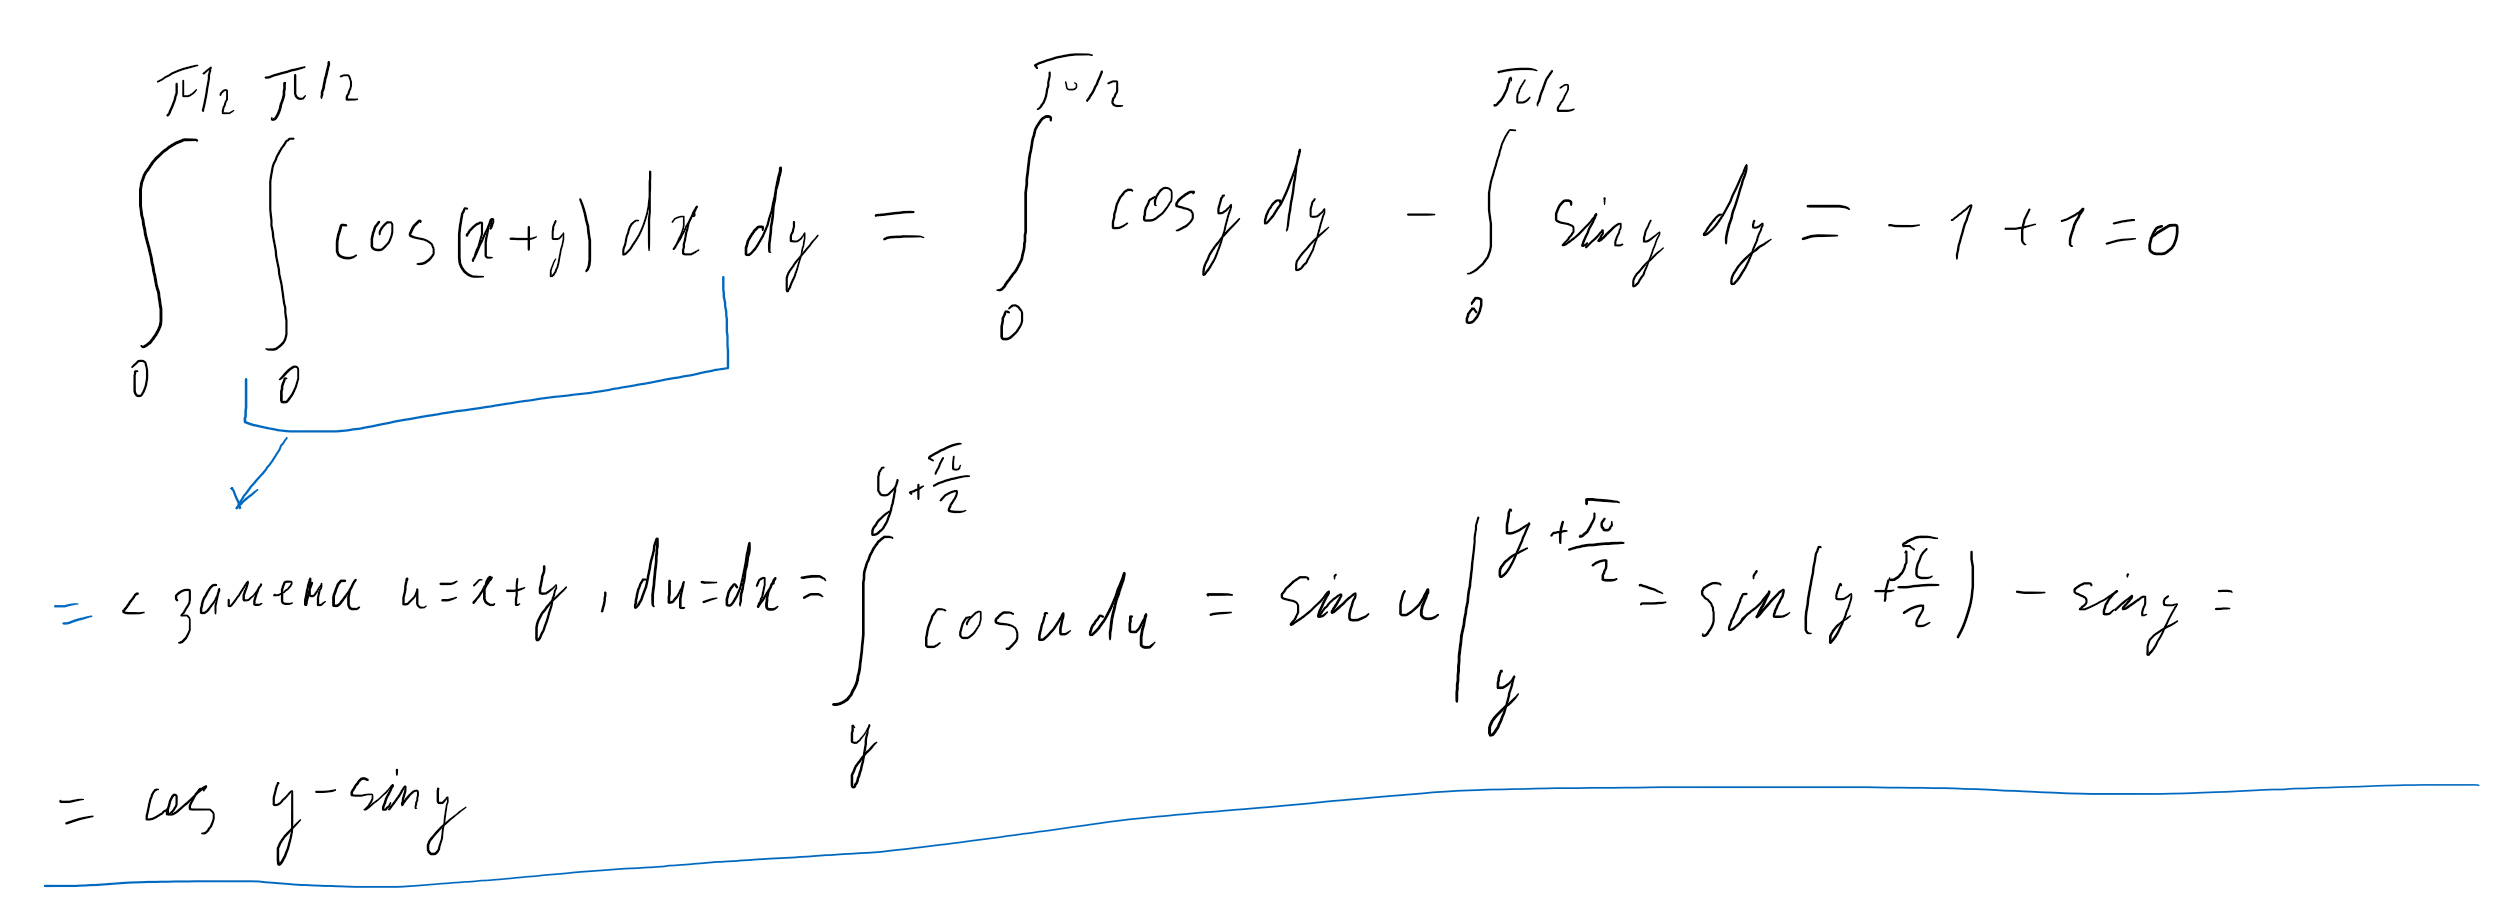
\includegraphics[width=\textwidth]{img/2asolve.png}


\textbf{Ответ: $0$}

\item 
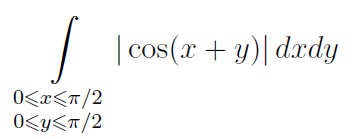
\includegraphics[scale=0.5]{img/2b.PNG}

\textbf{Решение:}\\

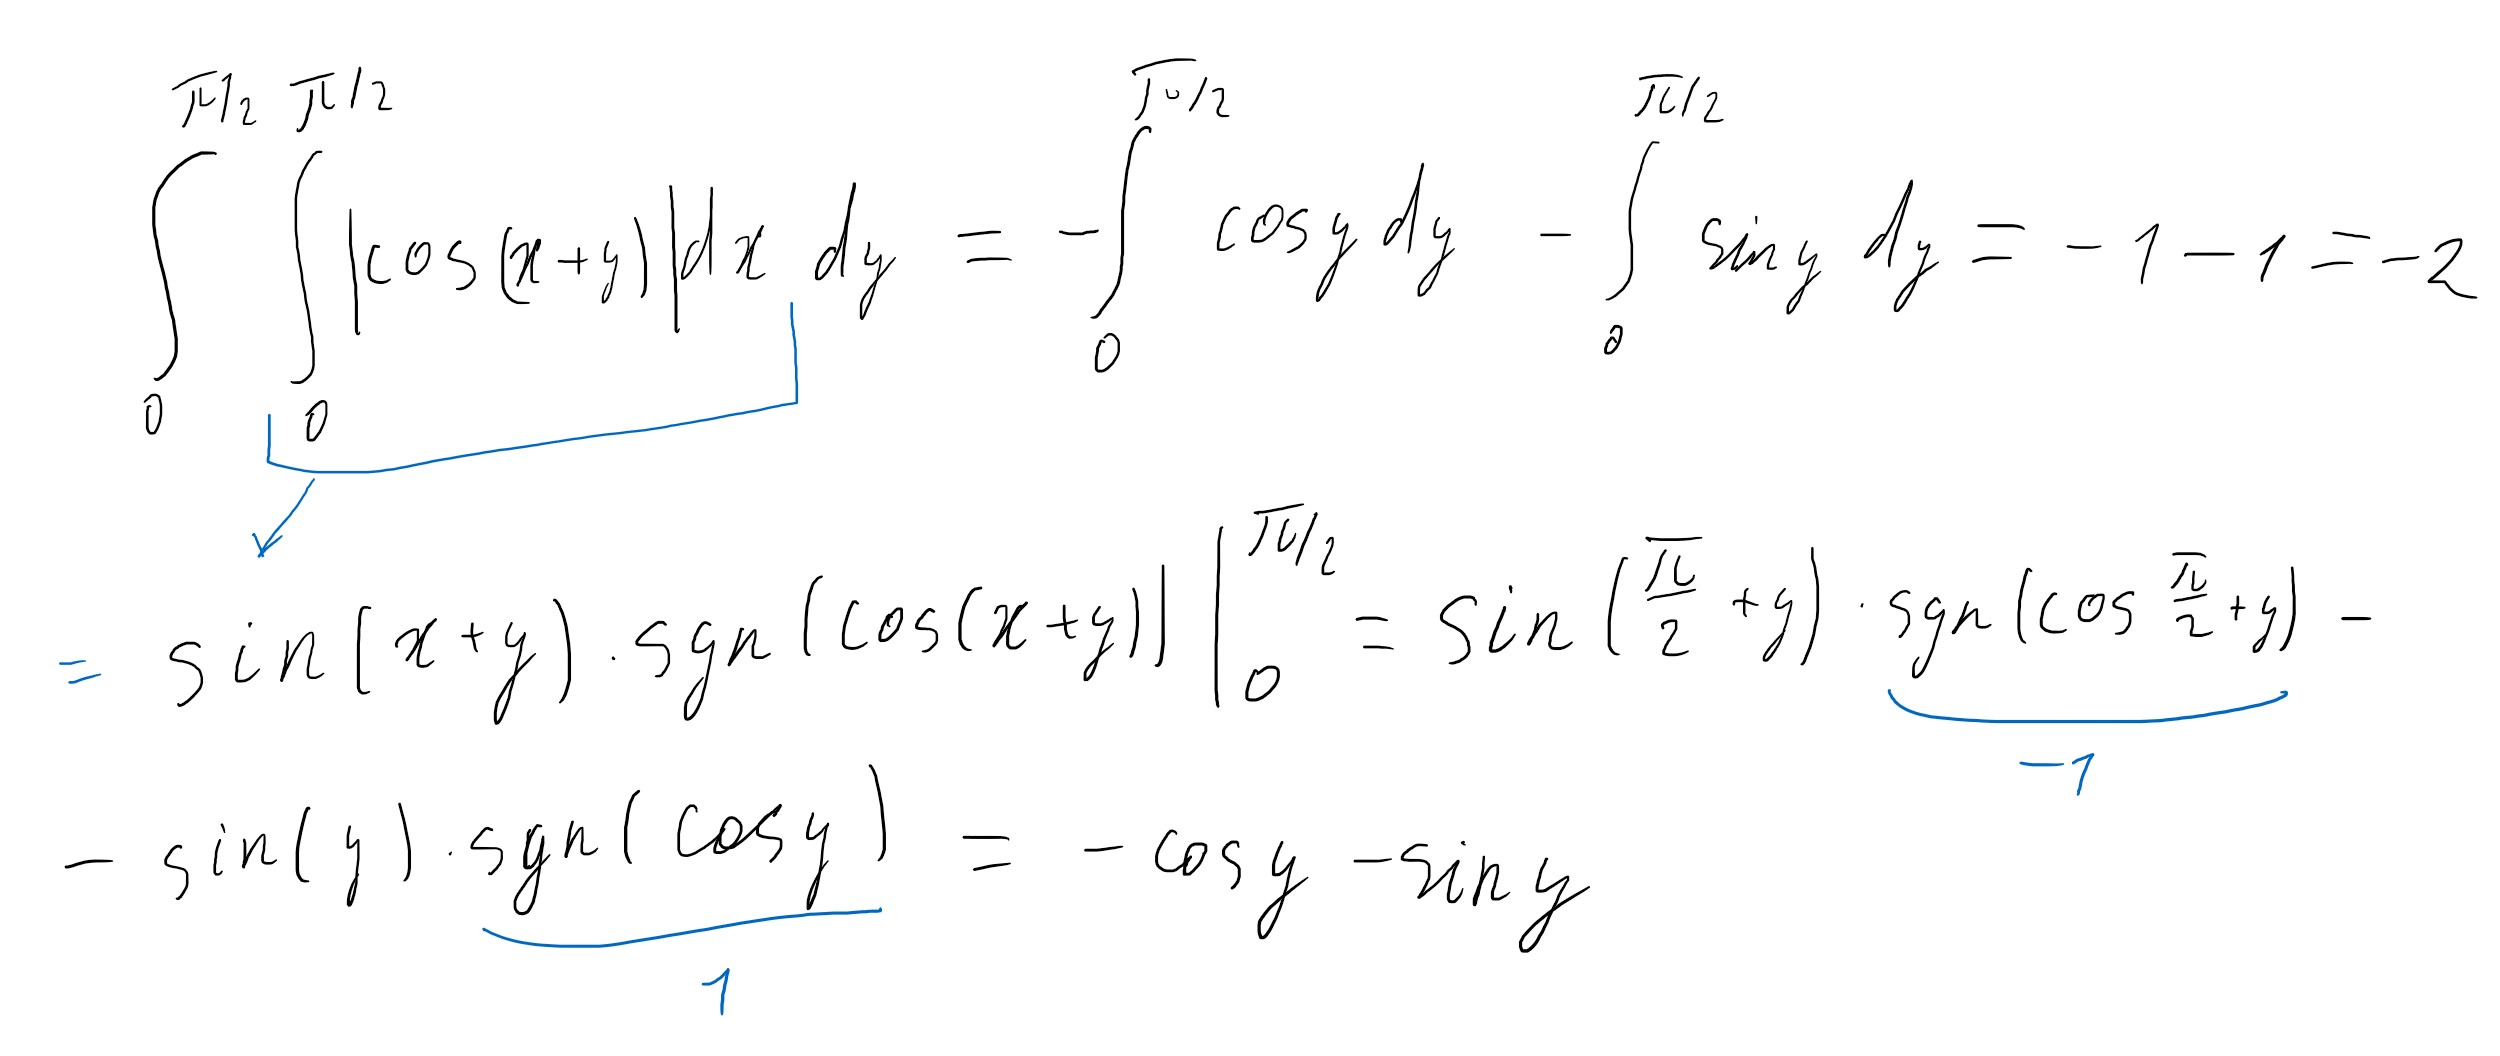
\includegraphics[width=\textwidth]{img/2bsolve.png}

\textbf{Ответ: $-2$}

\end{enumerate}

\item Найдите точки условного экстремуму

\begin{enumerate}

\item $z=xy$ при $x+y=1$

\textbf{Решение:}\\
Составим Лагранжиан:

$$L= \alpha(xy)-\lambda(x+y -1)$$
$$\frac{\partial L}{\partial x} = \alpha y-\lambda =0$$
$$\frac{\partial L}{\partial y} = \alpha x-\lambda =0$$

Решением систему уравнений $\begin{cases} \frac{\partial L}{\partial x}=0 \\ \frac{\partial L}{\partial y}=0\end{cases}$ будет или $\alpha =\lambda = 0$ или $a\neq0, x=y=\frac{\lambda}{\alpha}$

Найдем точку $x=y$ на границе $x+y=1$. $2x=1; x=0.5$. Точка $(0.5,0.5)$

$z(0.5,0.5)=0.25$. Для другой точки - $z(5,-4)=-20$, $z(0.5,0.5)>z(5,-4)$ значит мы нашли максимум.

\textbf{Ответ: максимум в точке $(0.5,0.5)$}
\item $z=x/a+y/b$ при $x^2 + y^2=1$

\textbf{Решение:}\\
Составим Лагранжиан:

$$L= \alpha(x/a+y/b)-\lambda(x^2 + y^2 -1)$$
$$\frac{\partial L}{\partial x} = \frac{\alpha}{a} -2\lambda x =0$$
$$\frac{\partial L}{\partial y} = \frac{\alpha}{b} -2\lambda y =0$$

Решим систему уравнений:
$$\begin{cases} \frac{\alpha}{a} -2\lambda x =0 \\ \frac{\alpha}{b} -2\lambda y =0\end{cases} \Rightarrow \begin{cases} \alpha -2a\lambda x =0 \\ \alpha -2b\lambda y =0\end{cases}\Rightarrow \begin{cases} \alpha -2a\lambda x =0 \\ 2a\lambda x -2b\lambda y =0\end{cases}\Rightarrow \begin{cases} \alpha -2a\lambda x =0 \\y=\frac{ax}{b} \end{cases} $$

Подставим $y=\frac{ax}{b}$ в условие $x^2 + y^2=1$:

$$x^2 +\frac{a^2x^2}{b^2}=1 \Rightarrow b^2x^2 +a^2x^2=b^2 \Rightarrow x^2(a^2+b^2) =b^2\Rightarrow x=\frac{ \pm b}{\sqrt{a^2+b^2}}$$

Выразим y через x и запишем координаты 2 точке: $(\frac{ b}{\sqrt{a^2+b^2}},\frac{ a}{\sqrt{a^2+b^2}})$ и $(-\frac{ b}{\sqrt{a^2+b^2}},-\frac{ a}{\sqrt{a^2+b^2}})$. 

Заметим, что функция $z=x/a+y/b$ возрастает в направлении роста y и x, значит точка с положительными знаками - максимум.

\textbf{Ответ: максимум в точке $(\frac{ b}{\sqrt{a^2+b^2}},\frac{ a}{\sqrt{a^2+b^2}})$ и минимум в точке $(-\frac{ b}{\sqrt{a^2+b^2}},-\frac{ a}{\sqrt{a^2+b^2}})$}

\end{enumerate}

\ 

\item Какие $r$ и $h$ дают наибольший объем полуцилиндрической ванны, площади S?

\textbf{Решение:}\\
Сведем эту задачу к поиску максимума.
Площадь поверхности нашей фигуры равна площади одного круга и половине площади поверхности бока цилиндра: 

$S=\pi r^2 +\pi r h$.
Объем этой фигуры - равен половине объема цилиндра(высота на площадь торца) = $V=\frac{1}{2}\pi r^2 h$.
Нужно найти максимум V при фиксированной площади.
Составим Лагранжиан:

$$L= \alpha(\frac{1}{2}\pi r^2 h)-\lambda(\pi r^2 +\pi r h -S)$$
$$\frac{\partial L}{\partial r} =\alpha \pi r h - 2\lambda \pi r - \lambda \pi h =0$$
$$\frac{\partial L}{\partial h} = \frac{1}{2}\alpha \pi r^2 - \lambda \pi r =0$$

Нетривиальным решением этой системы уравнений $\begin{cases} \frac{\partial L}{\partial r}=0 \\ \frac{\partial L}{\partial h}=0\end{cases}$ будет $r=\frac{2\lambda}{\alpha}, h=\frac{4\lambda}{\alpha}$ при $\alpha\neq0, \lambda\neq0$. Это означает, что $h=2r$. Проверим, максимум это или минимум.
Сравним вариант $V(h=2r)$ и $V(h=r)$.

Подставим $h=r$ в формулу площади и выразим h и r через S. $h =r= \sqrt{\frac{S}{2\pi}}$ 

$$V(h=r)=\frac{1}{2}\pi \frac{S}{2\pi} \sqrt{\frac{S}{2\pi}}=\frac{S}{4\pi} \sqrt{\frac{S}{2\pi}}$$
Подставим $h=2r$ в формулу площади и выразим h и r через S. $ r= \sqrt{\frac{S}{3\pi}}$  и $ h= \frac{2\sqrt{S}}{\sqrt{3\pi}}$
$$V(h=2r)=\frac{1}{2}\pi \frac{S}{3\pi} \frac{2\sqrt{S}}{\sqrt{3\pi}}=\frac{S}{3\pi} \frac{\sqrt{S}}{\sqrt{3\pi}}$$

Сравним:
$$V(h=r) < V(h=2r) \Leftrightarrow \frac{S}{4\pi} \sqrt{\frac{S}{2\pi}}<\frac{S}{3\pi} \frac{\sqrt{S}}{\sqrt{3\pi}}\Leftrightarrow 3\pi \sqrt{3\pi} <4\pi \sqrt{2\pi}\Leftrightarrow3 \sqrt{3} <4 \sqrt{2} \Leftrightarrow 27<32$$ 
Из этого следует, что мы нашли максимум.


\textbf{Ответ: максимальный объем при фиксированной площади при  $h=2r$}

\item Найдите максимум и минимум функции  $z = x^2 + y^2 -12x +16y$ при условии $x^2 + y^2 \leq 25$

\textbf{Решение:}\\

${grad}_az = \big(2(x-6), 2(y+8)\big)$ и градиент равен 0 в точке $(6,-8)$, которая лежит вне окружности, радиуса 5, которая задана условием. Значит критические точки будут находится строго на границе $x^2 + y^2 = 25$.

Составим Лагранжиан:

$$L= \alpha(x^2 + y^2 -12x +16y)-\lambda(x^2 + y^2 -25)$$
$$\frac{\partial L}{\partial x} = 2\alpha(x-6)-2\lambda x =0$$
$$\frac{\partial L}{\partial y} = 2\alpha(y+8)-2\lambda y =0$$

Решением этой системы уравнений $\begin{cases} \frac{\partial L}{\partial x}=0 \\ \frac{\partial L}{\partial y}=0\end{cases}$ будет $y =-\frac{4x}{3}$ при $x\neq0$.

Совмещая это условие с $x^2 + y^2 = 25$, мы найдем 2 точки:
$(3,-4);(-3,4)$

$$z(3,-4)=-75$$
$$z(-3,4)=125$$
Мы нашли, какая точка минимум, какая максимум.

\textbf{Ответ: минимум в точке $(3,-4)$ и максимум в точке $(-3,4)$}

\end{enumerate}
\end{document}